\subsection*{Assignment 1}
\addcontentsline{toc}{subsection}{Assignment 1}
In the following, the code to answer the questions of the first assignment is plotted.

\subsubsection*{Task 1}
\addcontentsline{toc}{subsubsection}{Task 1}
\begin{lstlisting}
%% 1) Create a phantom for simulating XCT measurements.
% The phantom should contain % ellipses and polygons of varying intensity
% (use phantom() and augment the resulting
% image). Show an image of your phantom.
% Size of quadratic Phantom in pixels
img_width = 256;
img_length = img_width;
% Determine Ellipe count (min = 3)
num_ellipses = 6;
% Initialize array
E = zeros(num_ellipses,6);
% Get basic skull structure from phantom
[~,base] = phantom('Modified Shepp-Logan', img_width);
E(1:2,:) = base(1:2,:);
% Get remaining array size
[M,N] = size(E(3:end,:));
% Create random ellipse along boundaries
E(3:end,1) = rand(M,1);
E(3:end,2) = -0.2 + (0.3+0.3)*rand(M,1);
E(3:end,3) = -0.4 + (0.4+0.4)*rand(M,1);
E(3:end,4) = -0.4 + (0.4+0.4)*rand(M,1);
E(3:end,5) = -0.45 + (0.45+0.45)*rand(M,1);
E(3:end,6) =  180*rand(M,1);
% Build phantom only of ellipses
phntm = phantom(E,img_width);
% Increase inensity of pixels in a square of the matrix
phntm(img_width/2-16:img_width/2+16,img_width/2-16:img_width/2+16) =...
    phntm(img_width/2-16:img_width/2+16,img_width/2-16:img_width/2+16) + 0.5;
% visualize the phantom
figure; imagesc(phntm);
axis equal tight; colormap gray; colorbar; xlabel('x'); ylabel('y');
title('Random Shepp-Logan Phantom');
\end{lstlisting}
\newpage

\begin{figure}[htb!]
    \centering
    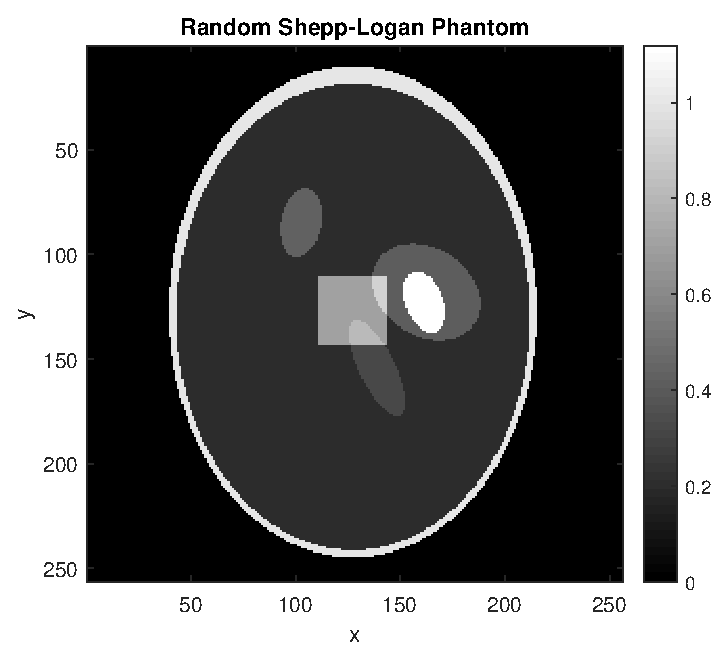
\includegraphics[width=\linewidth]{homework1/img/10.eps}
    \caption{Randomly generated skull}
    \label{fig:rand_skull}
\end{figure}

\clearpage
\newpage
\subsubsection*{Task 2}
\addcontentsline{toc}{subsubsection}{Task 2}

\begin{lstlisting}
%% 2) Compute the views (projections) for the range of angles from 0 to 179 degrees with spacing
% of 1, 5 and 10 degrees. Show the projections at 0, 30, 45 and 90 degrees (in one axes). Show the
% sinogram with the most angles/projections.
% specify projection angles
theta = {0:1:179;
    0:5:179;
    0:10:179}; 
% pad the image with zeros so nothing gets lost during rotation
img_diag = sqrt(img_length^2 + img_width^2);
padding = ceil(img_diag - img_width) + 4;
pad_img = zeros(img_length + padding, img_width + padding);
pad_img(ceil(padding/2):(ceil(padding/2) + img_length - 1),...
    ceil(padding/2):(ceil(padding/2) + img_width - 1)) = phntm;
% loop over the number of angles and summarize
th = theta{1};
n = length(th);
img_pr = zeros(size(pad_img,2), n);
for i = 1:n
    tmp_img = imrotate(pad_img,180+th(i), 'bilinear', 'crop');
    img_pr(:,i) = (sum(tmp_img))';
end
% create a sinograms for the specified angles
for i = 1:length(theta)
sinogram{i}(:,:) = radon(phntm, theta{i}); 
end
% Plot sinogram data at specific points in the same axes
figure;
plot(sinogram{1}(:,1),'DisplayName',[num2str(theta{1}(:,1))  ' degrees']);
hold on
plot(sinogram{1}(:,31),'DisplayName',[num2str(theta{1}(:,31)) ' degrees']);
plot(sinogram{1}(:,46),'DisplayName',[num2str(theta{1}(:,46)) ' degrees']);
plot(sinogram{1}(:,91),'DisplayName',[num2str(theta{1}(:,91)) ' degrees']);
title('Radon Transform at specific angles'); legend
% visualize the sinogram
figure; 
imagesc(sinogram{1}); 
title(['Sinogram @ ' num2str(length(theta{1})) 'angles (' num2str(theta{1}(:,1)) '\textdegree -' num2str(theta{1}(:,end)) '\textdegree)']);
xlabel('Angle');colormap gray;colorbar
\end{lstlisting}

\begin{figure}[htb!]
    \centering
    \includegraphics[width=.6\linewidth]{homework1/img/8.eps}
    \caption{Sinogram with the most angles (180)}
    \label{fig:sinogram:compl_angles}
\end{figure}

\begin{figure}[htb!]
    \centering
    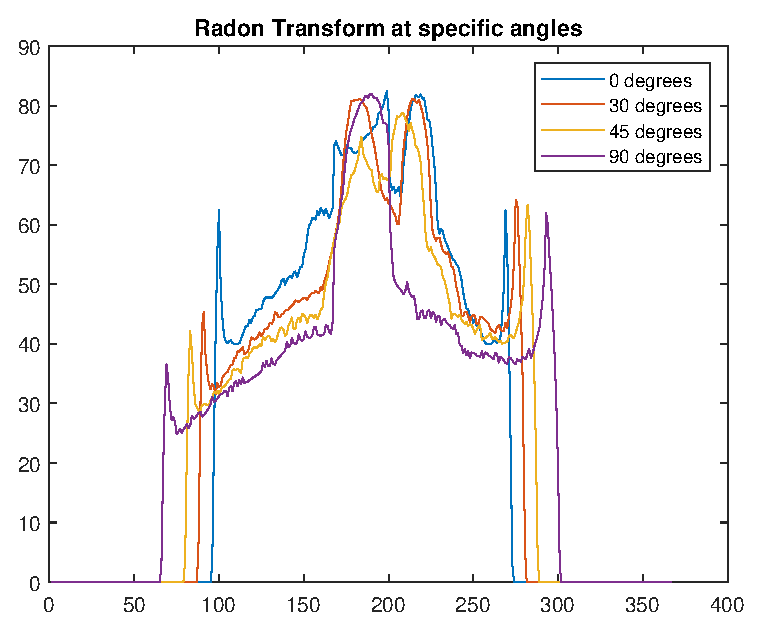
\includegraphics[width=.6\linewidth]{homework1/img/9.eps}
    \caption{Projections at the specific angles}
    \label{fig:sinogram:spec_angles}
\end{figure}

\clearpage
\newpage

\subsubsection*{Task 3}
\addcontentsline{toc}{subsubsection}{Task 3}

The following code was implemented as a seperate MATLAB function, in order to reduce the amount and simplify the code.

\begin{lstlisting}
%%%%%%%%%%%%%%%%%%%%%%%%%%%%%%%%%%%%%%%%%%%%%%%%%%%%%%%%%%%%%%%%%%%%%%%%%%%
%% Backprojection Algorithm %%
%%%%%%%%%%%%%%%%%%%%%%%%%%%%%%%%%%%%%%%%%%%%%%%%%%%%%%%%%%%%%%%%%%%%%%%%%%%
% Parameters: 
% sinogram: Input 2D - sinogram matrix
% theta: corresponding angles of sinogram
% filter_shape('none','Ramp','Cos','Hamming'): Selection of applied filter
% method
% Output: 
% rec: Reconstructed image
function rec = backprojection(sinogram,theta,filter_shape)
if nargin <3
    filter_shape = 'none';
end
% figure out how big the picture is going to be.
sideSize = size(sinogram,1); 
%filter setups
x = linspace(-1,1,sideSize);
ramp = abs(x);
switch filter_shape
    case 'Ramp'
        filter = ramp;
    case 'Hamming'
        filter = ramp .* hamming(sideSize)';
    case 'Cos'
        filter = ramp .* cos((x./2).*pi).^2;
    otherwise
        filter = 1;
end
% set up the image
rec = zeros(sideSize,sideSize);
for i = 1:length(theta)    
    line = sinogram(:,i);    
    % perform fft
    line_fft = fftshift(fft(ifftshift(line)));        
    % filter in frquency space
    line_fft_filtered = line_fft .* filter';    
    % transform back into time domain
    line_filtered = ifftshift(ifft(fftshift(line_fft_filtered)));    
    % backproject
    image = repmat(line_filtered,1,sideSize);
    image = imrotate(image,theta(i),'crop');    
    % sum up final picture
    rec = rec + image;
end
% rotate image as the original
rec = real(imrotate(rec,90))./length(theta);
end
\end{lstlisting}


\clearpage
\newpage


\subsubsection*{Task 4}
\addcontentsline{toc}{subsubsection}{Task 4}

\begin{lstlisting}
%% 4) Reconstruct the phantom data with the specified angular spacings using your
% backprojection algorithm without filtering. Show the obtained reconstructions.
recon = backprojection(sinogram{1},theta{1});
% visualize reconstruction results
figure;
subplot(1,2,1);
imagesc(phntm);
axis equal tight;
colormap gray;
title('Original'); xlabel('x'); ylabel('y');
subplot(1,2,2);
imagesc(recon);
axis equal tight;
colormap gray;
title('Unfiltered BP'); xlabel('x'); ylabel('y');
\end{lstlisting}
\begin{figure}[htb!]
  \centering
  \includegraphics[width=\linewidth]{homework1/img/7.eps}
  \caption{Reconstruction from 1\textdegree resolution without any filtering}
  \label{fig:recon_1deg}
\end{figure}

\clearpage
\newpage


\subsubsection*{Task 5}
\addcontentsline{toc}{subsubsection}{Task 5}

\begin{lstlisting}
%% 5) Incorporate filtering in your backprojection. Implement 3 filters (ramp, cosine and
% hamming) and test their influence on the reconstruction using your phantom data (pick
% a single angle spacing). Show the reconstruction results
for i = 1:3
    % Compute filtered backprojections
    recon_cos = backprojection(sinogram{i},theta{i},'Cos');
    recon_ramp = backprojection(sinogram{i},theta{i},'Ramp');
    recon_hamming = backprojection(sinogram{i},theta{i},'Hamming');
    % visualize reconstruction results
    figure;
    subplot(2,2,1);
    imagesc(phntm);
    title(['w/o Filtering,' num2str(length(theta{i})) ' angles']);
    colormap gray; colorbar; xlabel('x'); ylabel('y');
    subplot(2,2,2);
    imagesc(recon_ramp);
    title(['w/ Ramp Filtering, ' num2str(length(theta{i})) ' angles']);
    colormap gray; colorbar; xlabel('x'); ylabel('y');
    subplot(2,2,3);
    imagesc(recon_hamming);
    title(['w/ Hamming Filtering, '  num2str(length(theta{i})) ' angles']);
    colormap gray; colorbar; xlabel('x'); ylabel('y');
    subplot(2,2,4);
    imagesc(recon_cos);
    title(['w/ Cosine Filtering, ' num2str(length(theta{i})) ' angles']);
    colormap gray; colorbar; xlabel('x'); ylabel('y');
end
\end{lstlisting}

\begin{figure}[htb!]
  \centering
  \includegraphics[width=\linewidth]{homework1/img/6.eps}
  \caption{1\textdegree resolution}
  \label{fig:recon_1deg}
\end{figure}
\begin{figure}[htb!]
  \centering
  \includegraphics[width=\linewidth]{homework1/img/5.eps}
  \caption{5\textdegree resolution}
  \label{fig:recon_5deg}
\end{figure}
\begin{figure}[htb!]
  \centering
  \includegraphics[width=\linewidth]{homework1/img/4.eps}
  \caption{10\textdegree resolution}
  \label{fig:recon_10deg}
\end{figure}


\clearpage
\newpage


\subsubsection*{Task 6}
\addcontentsline{toc}{subsubsection}{Task 6}

\begin{lstlisting}
%% 6) Reconstruct the provided datasets (CT_2018.mat) with your backprojection algorithm
% without filtering and with each of the implemented filters, respectively. Show the
% reconstructed images.

% load sample data
S = load('CT_2018.mat');
% loop over sample data, compute backprojections and plot them each in a
% single figure
for i = 1:3
    % change variable name dynamically
    sino_name = S.(['sino' num2str(i-1)]);
    angle = S.(['theta' num2str(i-1)]);
    % visualize
    fig_name = sprintf('%s with %d angles from %d° to %d°', ['sino' num2str(i-1)],length(angle), angle(1),angle(end));
    figure('Name',fig_name);
    subplot(2,2,1);
    recon = backprojection(sino_name,angle);
    imagesc(recon);
    title('w/o Filtering');
    colormap gray; colorbar; xlabel('x'); ylabel('y');
    subplot(2,2,2);
    recon = backprojection(sino_name,angle,'Ramp');
    imagesc(recon);
    title('w/ Ramp Filtering');
    colormap gray; colorbar; xlabel('x'); ylabel('y');
    subplot(2,2,3);
    recon = backprojection(sino_name,angle,'Hamming');
    imagesc(recon);
    title('w/ Hamming Filtering');
    colormap gray; colorbar; xlabel('x'); ylabel('y');
    subplot(2,2,4);
    recon = backprojection(sino_name,angle,'Cos');
    imagesc(recon);
    title('w/ Cosine Filtering');
    colormap gray; colorbar; xlabel('x'); ylabel('y');
end
\end{lstlisting}

\begin{figure}[htb!]
  \centering
  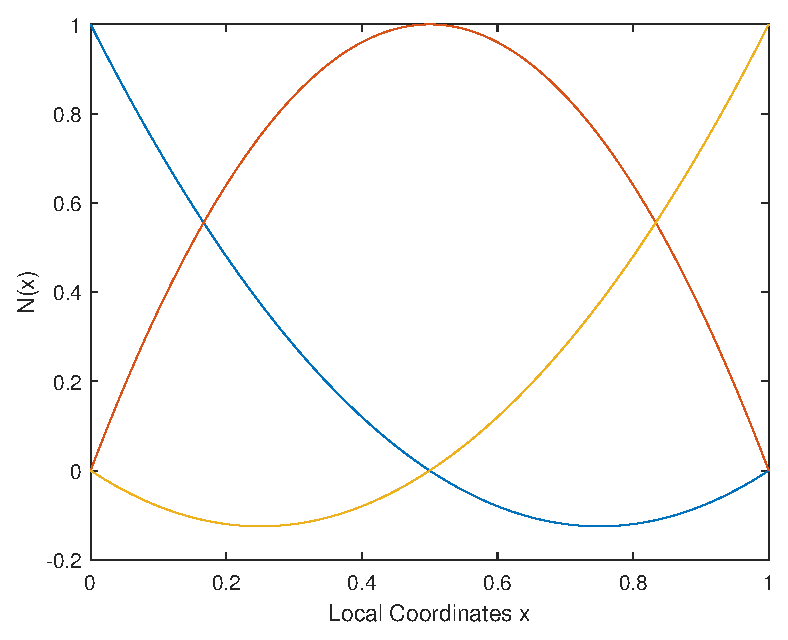
\includegraphics[width=\linewidth]{homework1/img/3.eps}
  \caption{1\textdegree resolution}
  \label{fig:recon_1deg}
\end{figure}
\begin{figure}[htb!]
  \centering
  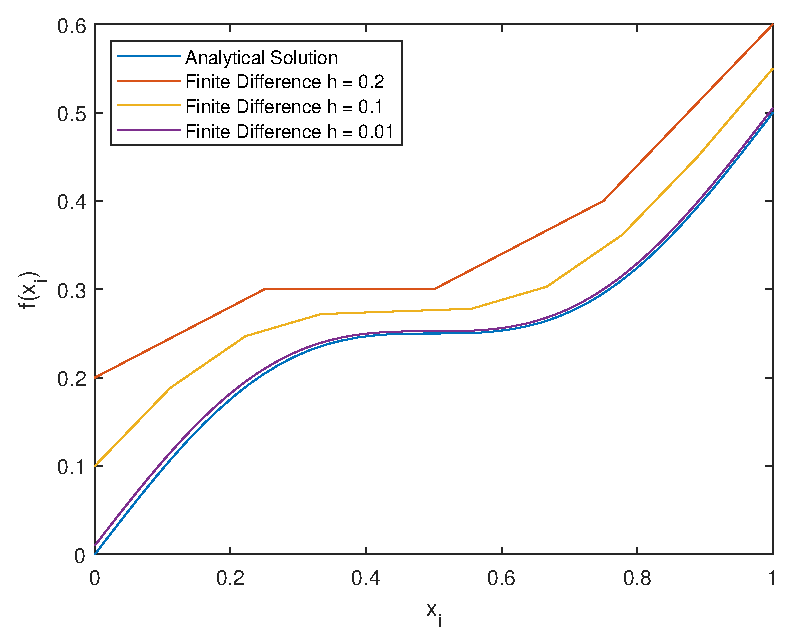
\includegraphics[width=\linewidth]{homework1/img/2.eps}
  \caption{2\textdegree resolution}
  \label{fig:recon_5deg}
\end{figure}
\begin{figure}[htb!]
  \centering
  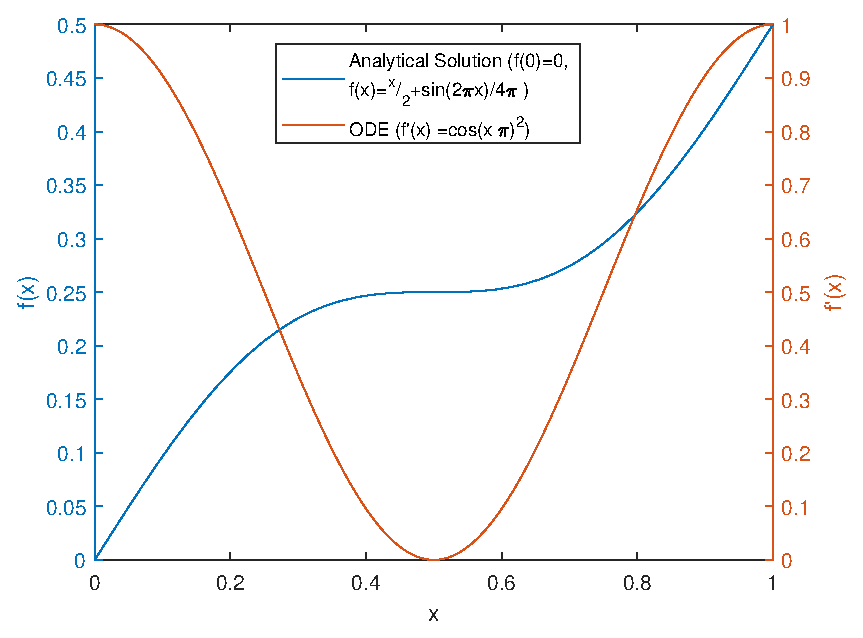
\includegraphics[width=\linewidth]{homework1/img/1.eps}
  \caption{0.5\textdegree resolution}
  \label{fig:recon_10deg}
\end{figure}

\clearpage
\newpage


\subsubsection*{Task 7}
\addcontentsline{toc}{subsubsection}{Task 7}

\textbf{Shortly interpret your results:}
\begin{enumerate}[label=(\alph*)]

\item What is the effect of different angular spacings on the reconstruction?\\
Finer Spacings <==> More Information, therefore better reconstruction, more details visible.

\item How do the different filters change the reconstruction results?\\
Filters affect the edge sharpness, the residual noise and the overall brightness of an image

\item Which filter performs best? Why? Under which circumstances?\\
The Hamming filter performs best overall, because he does not damp the low frequencies to zero,as cosine and ramp filter do.
\end{enumerate}

\begin{enumerate}[label=(\alph*)]
    \item What is the effect of different angular spacings on the reconstruction?\\
    Finer spacing provide more information, therefore a better reconstruction is possible.
    \item How do the different filters change the reconstruction results?\\
    Different filters affect different radial resolutions. They either provide more or less noise.
    \item Which filter performs best? Why? Under which circumstances?\\
    In the case of the self-made phantom, the Hamming filter performs best due to its elaborate filtering function. In comparison of the three filters the hamming flter is a good compromise between high contrast and noise. The cos filter looses a lot of information for low frequencies. Filtering is always a trade off between reducing the noise and getting a high resolution.
\end{enumerate}

